\section{\secrel}
\label{sec_relations}

All mathematics can be built from sets. A key step is to use sets to define relations.  Functions and operations are examples of relations, but that is just the tip of the iceberg. Almost every mathematical symbol you know is either the name of a set or a relation. For example, each of the following mathematical symbols represents a relation
    $$+ \quad \times \quad \sqrt{~} \quad \mid \quad = \quad \neq \quad \le \quad > \quad \land \quad \lor \quad \cap \quad \cup \quad \oplus \quad \in \quad \subseteq \quad \sim \quad \cong \quad \equiv  \quad \| \quad \perp$$
Relations are built from the Cartesian product of sets, so we begin there.  
%%%%%%%%%%%%%%%%%%%%

\newcommand{\subcartprod}{The Cartesian Product of Sets}
\subsection{\subcartprod}
\label{sub_cart_prod}

The Cartesian product of sets is another set operation that we can use to build new sets from known sets. The Cartesian product of two sets is defined using ordered pairs, which we define in \Cref{defn_ordered_pairs}. It is useful to form the Cartesian product of any finite number of sets. For that, we need to extend the definition to ordered tuples of any finite length.

\begin{defn}[Ordered tuples]
\label{defn_ordered_tuple}
~
    \begin{apart}
        \item For sets $X_1$, $X_2$, $X_3$,\ldots, $X_n$ and elements $x_1\in X_1$, $x_2\in X_2$, $x_3\in X_3$, \ldots, $x_n\in X_n$, the \vocab{ordered $n$ tuple} $(x_1,x_2,x_3, \ldots, x_n)$ is defined by 
            $$(x_1,x_2, x_3, \ldots, x_n) = \{\{x_1\}, \{x_1,x_2\}, \{x_1,x_2,x_3\}, \ldots, \{x_1,x_2,x_3,\ldots, x_n\}\}$$
        For example, if $X_1=X_2=X_3=\mathbb{Z}$, then      \
            $$(1,5,2) = \{\{1\}, \{1,5\}, \{1,2,5\}\}$$ 
        whereas 
            $$(2,1,5) = \{\{2\}, \{1,2\}, \{1,2,5\}\}.$$
        \item In the ordered tuple $(x_1,x_2,x_3, \ldots, x_n)$, we say that $x_1$ is the \vocab{first coordinate}, $x_2$ is the \vocab{second coordinate}, $x_3$ is the \vocab{third coordinate}, \ldots, $x_n$ is the $n^{\text{th}}$ \vocab{coordinate}.  For example, in $(1,5,2)$, the first coordinate is 1, the second coordiante is 5, and the third coordinate is 2.
    \end{apart}
\end{defn}

In applications to databases, the coordinates often come from different sets.  

\begin{exam}[Ordered tuples of data]
\label{exam_ordered_tuples_data}
    Create 4-tuples to represent each student at a university where the first coordinate is the student's first name, the second coordinate is that student's family name, the third coordinate is the number of credit hours the student has completed, and the fourth coordinate indicates if the student lives on-campus or off-campus.
        \begin{soln}
            Let $X_1=X_2$ be the set of all alphabetic strings of length up to ten (for the names), let $X_3=\{0,1,2,3,\ldots, 999\}$ (for the completed credit hours), and $X_4=\{\bs{0},\bs{1}\}$ (for off-campus and on-campus, in that order). For example, the student Elizabeth Anderson who has completed 48 credit hours and currently lives off-campus might be represented by the the 4-tuple $$(\str{Elizabeth}, \str{Anderson}, 48,\bs{0}).$$
        \end{soln}
\end{exam}

We are now ready to define the Cartesian product of sets.

\begin{defn}[Cartesian product of sets]
\label{defn_cart_prod_sets}
~
    \begin{apart}
        \item Given sets $X$ and $Y$, the \vocab{Cartesian product}, denoted $X \times Y$, is the set of all ordered pairs of the form $(x,y)$ where $x \in X$ and $y\in Y$.  That is,
            $$X \times Y = \{ (x,y) \mid x \in x \text{ and } y \in Y \}.$$
        For example, if $X = \{2,3,5\}$ and $Y = \{0,1\}$, then 
            $$X \times Y = \{ (2,0), (2,1), (3,0), (3,1), (5,0), (5,1)\}.$$ 
        
        \item Similarly, given sets $X_1$, $X_2$, $X_3$, \ldots, $X_n$, the \vocab{Cartesian product}, denoted $X_1 \times X_2 \times X_3 \times \cdots \times X_n$, is the set of all ordered $n$-tuples of the form $(x_1, x_2, x_3,\ldots, x_n)$ where $x_1 \in X_1$, $x_2 \in X_2$, $x_3 \in X_3$, \ldots, $x_n \in X_n$.  That is,
            $$X_1 \times X_2 \times X_3 \times \cdots \times X_n = \{(x_1, x_2, x_3, \ldots, x_n) \mid x_1 \in X_1, x_2 \in X_2, x_3 \in X_3, \ldots, x_n \in X_n\}.$$
        For example, if $X_1=\{0,1\}$, $X_2=\{a,b\}$, and $X_3 = \{1,2\}$, then
            $$X_1 \times X_2 \times X_3= \{ (0,a,1), (0,a,2), (0,b,1), (0,b,2), (1,a,1), (1,a,2), (1,b,1), (1,b,2)\}.$$

        \item We are often interested in the Cartesian product of a set with itself.  Given a set $X$ we write 
            $$X^n=\underbrace{X \times X \times X \times \cdots \times X}_{n \text{ times}}.$$
        For example, $\mathbb{R}^2$ is the usual $xy$-plane and $\mathbb{R}^3$ is the usual $xyz$-space.
    \end{apart}
\end{defn}

If the elements of the sets $X$ and $Y$ are real numbers, then $S \times T \subseteq \mathbb{R}^2$ and so we can draw $X \times Y$ as points in the $xy$-plane.

\begin{exam}[Drawing the Cartesian product of two sets of real numbers as points in the $xy$-plane]
    Consider the sets $X = \{2,3,5\}$ and $Y = \{0,1\}$ from \Cref{defn_cart_prod_sets}.  Draw $X \times Y$ as points in the $xy-$plane.
        \begin{soln}
            We plot the points of $X \times Y$ in \Cref{fig_cart_prod_as_points}.

            \begin{figure}[hbtp]
                \centering
                %Used in \Cref{sub_cart_prod}

\begin{tikzpicture}[point/.style={fill,circle,inner sep=2.5pt,black}]
  \draw[latex-latex] (-1,0) -- (6.5,0)node[right]{$x$};
  \foreach \x [evaluate=\x as \lab using int(\x)] in {1,2,3,4,5,6}{
    \draw[thin](\x,-0.1)--node[below=1mm]{$\lab$}++(0,0.2); % draw ticks x-axis
  }
    \draw[latex-latex] (0,-1) -- (0,2.5)node[above]{$y$};
    \foreach \x [evaluate=\x as \lab using int(\x)] in {1,2}{
    \draw[thin](-0.1,\x)--node[left=1mm]{$\lab$}++(0.2,0);  % draw ticks y-axis
  }
  \node[point] at (2,0){}; 
    \node[point] at (3,0){}; 
      \node[point] at (5,0){}; 
  \node[point] at (2,1){}; 
    \node[point] at (3,1){}; 
      \node[point] at (5,1){}; 
\end{tikzpicture}
                \caption{Representing $\{2,3,5\} \times \{0,1\}$ as points in the $xy$-plane.}
                \label{fig_cart_prod_as_points}
            \end{figure}
        \end{soln}
\end{exam}

Your turn to work with ordered pairs, ordered tuples, and the Cartesian product of sets.

\begin{act}[Cartesian product]
\label{act_cart_prod}
~
    \begin{actpart}
        \item Consider the sets $P = \{0,1,2,3\}$ and $Q = \{1,5,7\}$. Give an example of an element in $P \times Q$ and an element in $Q \times P$.  Is there any ordered pair in both $P \times Q$ and $Q \times P$?
        \item Again, consider the sets $P = \{0,1,2,3\}$ and $Q = \{1,5,7\}$. Represent $P \times Q$ as points in the $xy$-plane and then represent $Q \times P$ as a set of points in the $xy$-plane.
        \item Conjecture how $|X \times Y|$ is related to $|X|$ and $|Y|$ when $X$ and $Y$ are finite sets.
        \item For the set $Q = \{1,5,7\}$, list the elements of $Q^2$ and represent $Q^2$ as a set of points in the $xy$-plane. 
        \item For the set $P = \{0,1,2,3\}$, give an example of an element of $P^3$.  How many elements does $P^3$ have?
        \item Conjecture how $|X^n|$ is related to $|X|$ when $X$ is a finite set.
    \end{actpart}
\end{act}

%%%%%%%%%%%%%%%%%%%%

\newcommand{\subfncartprod}{Functions Involving Cartesian Products}
\subsection{\subfncartprod}
\label{sub_fn_cart_prod}

Note that the domain and/or codomain of a function can be a Cartesian product.  A quick note on notation when the domain is a Cartesian product

\begin{rem}[Notation for Functions on Cartesian products]
\label{rem_fn_on_cart_prod}
    For sets $X_1$, $X_2$, \ldots $X_n$, if we have a function $f$ with domain $X_1 \times X_2 \times \cdots \times X_n$, then we should write $f((x_1,x_2, \ldots, x_n))$ where each $x_i \in X_i$, but the double parentheses look silly, so we often write $f(x_1,x_2, \ldots, x_n)$ instead.
\end{rem}

Here are some examples of functions involving Cartesian products of sets.

\begin{exam}[Functions involving Cartesian products of sets]
~
    \begin{actpart}
        \item Consider the function $f: \mathbb{R}^2 \to \mathbb{R}$ defined by $f(x,y) = x+y$.  Identify the domain and codomain of $f$, evaluate $f(3,4)$, and describe the set of all ordered pairs $(x,y)$ with $f(x,y)=0$ as a set of points in the $xy$-plane.
            \begin{soln}
                The domain of $f$ is $\mathbb{R}^2$ and the codomain is $\mathbb{R}$. 
                Next, $f(3,4) = 3+4 = 7$.  To find all points with $f(x,y)=7$ we solve $x+y=7$ to get $y = 7-x$ which is the line with slope -1 and $y$-intercept 7.
                \end{soln}
        
        \item Consider the function $g: \{0,1,2,3\} \to \{1,2,3,4\} \times \{0,1,2,\ldots,10\}$ defined by $g(a) = (a+1,a^2)$.  Identify the domain and codomain of $g$, evaluate $g(0)$ and $g(3)$, and describe the image of $g$.
            \begin{soln}
                The domain is $\{0,1,2,3\}$ and the codomain is $\{1,2,3,4\} \times \{0,1,2,\ldots,10\}$.  We evaluate $g(0) = (0+1,0^2)=(1,0)$ and $g(3) = (3+1,3^2)=(4,9)$.  There are only finitely many integers in the domain so we can find the image by listing the values 
                    $$\{g(0), g(1), g(2), g(3) \} = \{ (1,0), (2,1), (3,4), (4,9)\}.$$
                You can confirm each of these ordered pairs is in the codomain, as required.
            \end{soln}
        \item Consider the function $h: \mathbb{Z}^2 \to \mathbb{Z}^2$ defined by $h(a,b) = (c,d)$ where $d=\fn{gcd}(a,b)$ and $m =\fn{lcm}(a,b)$, the least (smallest) integer that it a common multiple of $a$ and $b$.  Identify the domain and codomain of $h$, evaluate $h(4,6)$, and describe all fixed points of the function $h$.  
            \begin{soln}
                The domain is $\mathbb{Z}^2$ and the codomain is also $\mathbb{Z}^2$.  We evaluate $h(4,6)=(2,12)$. The fixed points of $h$ are the points $(a,b)$ where $h(a,b) = (a,b)$. It follows that $a$ is a common divisor of $a$ and $b$ and $b$ is a common multiple of $a$ and $b$.  That happens exactly when $a \mid b$, so $(a,b)$ is a fixed point exactly when $a \mid b$. 
            \end{soln}
    \end{actpart}
\end{exam}

As usual, the domain and codomain of functions can involve any type of discrete object.

\begin{exam}[Functions involving Cartesian products and discrete objects]
\label{exam_cart_prod_fn_discrete}
~
    \begin{apart}
        \item Let $S = \{0,1,2,3\}$ and, as usual, let $\mathscr{P}(S)$ denote the set of all subsets of $S$. Consider the function $\fn{int}: \mathscr{P}(S)^2 \to \mathscr{P}(S)$ defined by $\fn{int}(A,B) = A \cap B$.  Evaluate $\fn{int}(\{0,1,2\},\{2,3\})$.
            \begin{soln}
                We have $\fn{int}(\{0,1,2\},\{2,3\}) = \{0,1,2\} \cap \{2,3\} = \{2\}.$
            \end{soln}
        
        \item Let $D=\{0,1,2,\ldots,9\}$ be the set of digits and let $$T=\{000,001,002,\ldots, 998, 999\}$$ be the set of all strings of digits of length three, the numbers 0-999 written as three-digit numbers. Consider the function $\fn{split}:T \to \mathbb{D}^3$ defined by $\fn{split}(abc)= (a,b,c).$  Evaluate $\fn{split}(486)$.
            \begin{soln}
                We get $\fn{split}(486)=(4,8,6)$.
            \end{soln}
    \end{apart}
\end{exam}

Try to work with functions involving Cartesian products

\begin{act}[Functions involving Cartesian products]
\label{act_fn_cart_prod}
    Consider the function $f: \mathbb{Z}^2 \to \mathbb{Z}$ defined by $f(a,b) = ab$. 
    \begin{actpart}
      \item State the domain and codomain of $f$ and evaluate $f(3,4)$.
      \item \label{part_another_pair_mult12} Give an example of an ordered pair $(a,b)$ different from $(3,4)$ with $f(a,b) = f(3,4)$.  What does that tell you about the function $f$?
      \item \label{part_mult_onto} Given any real number $n$, find an ordered pair $(a,b)$ such that $f(a,b)=n$.  Hint: Write $a$ and $b$ in terms of $n$. What does that tell you about the function $f$?
      \item For a given integer $n$, how many ordered pairs $(a,b)$ have $f(a,b)=n$?  Hint: Do not forget the negative divisors. 
    \end{actpart}
\end{act}

%%%%%%%%%%%%%%%%%%%%

\newcommand{\subdefnrelation}{Relations and Their Representations}
\subsection{\subdefnrelation}
\label{sub_defn_relation}

We are now ready to define a relation.

\begin{defn}[Relation]
\label{defn_relation}
~
    \begin{apart}
        \item For any sets $X$ and $Y$, a \vocab{relation (from X to Y)} is a subset of $X \times Y$.  For example, the set $R=\{(a,0),(a,1),(b,1),(b,2)\}$ is a relation from $\{a,b\}$ to $\{0,1,2\}$.
        \item In many of the important examples, $X=Y$, and we just say $R$ is a \vocab{relation on $X$}.  For example, the set $R=\{(0,0),(0,1),(0,2),(1,1),(1,2),(2,2)\}$ is  relation on $\{0,1,2\}$.  We could equivalently define $R = \{(a,b) \mid a, b \in \{0,1,2\} \text{ and } a \le b\}.$
    \end{apart}
\end{defn}

Note that the graph of any function is a relation. 

\begin{defn}[Graph of a function]
\label{defn_graph_fn}
    For sets $X$ and $Y$ and function $f: X \to Y$, the \vocab{graph of the function} $f$ is the relation
    $$\{(x,y) \mid x \in X, y \in Y, \text{ and } y = f(x)\}$$ or, equivalently, the graph of $f$ is $$\{(x,f(x)) \mid x \in X\}.$$
    For example, if $f: \mathbb{R} \to \mathbb{R}$ is the function defined by $f(x) = 2x+1$, then the graph of $f$ is the line $y=2x+1$ that has slope two and intercept one.
\end{defn}

More generally, any graph in the $xy$-plane is a relation on $\mathbb{R}$.  For example, the unit circle $U = \{ (x,y) \mid x^2+y^2=1\}$ shown in \Cref{fig_unit_circle_verticallinetest} is a relation.  

Although every function has a graph that is a relation, not every relation is the graph of a function.  For example, we see in \Cref{exam_when_graph_is_fn} that the unit circle is not the graph of a function.

Let's look at another example of the graph of a function.

\begin{exam}[The graph of a function on $\mathbb{Z}$.]
\label{exam_graph_fn_is_relation}
    Consider the function $s: \mathbb{Z} \to \mathbb{Z}$ defined by $s(n) = n^2+1$ and let $R$ be the graph of $s$.
       \begin{apart}
           \item   Is $(3,8) \in R$?  Is $(2,5) \in R$?
               \begin{soln}
                   Since $s(3) = 3^2+1=10 \neq 8$, it follows that $(3,8)$ is not on the graph of $s$ and so $(3,8) \notin R$.  On the other hand, since $s(2) = 2^2+1=5$, it follows that $(2,5)$ is on the graph of $s$ and so $(2,5) \in R$.
               \end{soln}
            \item Find all integers $m \in \mathbb{Z}$ such that $(2,m) \in R$ and find all integers $n \in \mathbb{Z}$ such that $(n,5) \in R$.
                \begin{soln}
                    First, if $(2,m) \in R$, then $m = s(2) = 5$.  No other value of $m$ is possible because by the definition of function (\Cref{defn_function}) there is only one value for $f(2)$.  Next, if $(n,5) \in R$, then $5 = f(n) = n^2 +1$.  Solving we get $n^2=4$ and so $n=2$ and $n=-2$.  
                \end{soln}
       \end{apart}
\end{exam}

When $X$ and $Y$ are finite sets or subsets of $\mathbb{Z}$, we have two ways to visually represent a relation from $X$ to $Y$.

\begin{defn}[Drawing relations on finite sets or subsets of $\mathbb{Z}$ using dot diagrams]
\label{defn_draw_relations_dot_diagrams}
~
    When $X$ and $Y$ are finite sets or subsets of $\mathbb{Z}$, we can represent a relation $R$ from $X$ to $Y$ using a \vocab{dot diagram} where we draw a vertex for each element of $X$ on the left and a vertex for each element of $Y$ on the right.  Then we draw an arrow from $x$ to $y$ if $(x,y) \in R$.  This is the same dot diagram we used to represent functions on a finite sets or subsets of $\mathbb{Z}$.  For example, the relation $R=\{(a,0),(a,1),(b,1),(b,2)\}$ from $\{a,b\}$ to $\{0,1,2\}$ can be represented using the dot diagram shown in \Cref{fig_relation_finite_dot_diagram}.
        \begin{figure}[hbtp]
            \centering
            %Used in \Cref{sub_defn_relation}.

\begin{tikzpicture}
[scale =.5]
\GraphInit[vstyle=Welsh]
\SetUpEdge[style={->,>=triangle 45}]
\SetGraphUnit{2}
%\SetVertexNoLabel
\Vertex[LabelOut,Lpos=180,x=0,y=3]{$a$}
\Vertex[LabelOut,Lpos= 180,x=0,y=1]{$b$}
\Vertex[LabelOut,Lpos=0,x=4,y=4]{$0$}
\Vertex[LabelOut,Lpos= 0,x=4,y=2]{$1$}
\Vertex[LabelOut,Lpos=0,x=4,y=0]{$2$}
\Edges($a$, $0$)
\Edges($a$, $1$)
\Edges($b$, $1$)
\Edges($b$, $2$)
\end{tikzpicture}
            \caption{The dot diagram for a relation on finite sets.}
            \label{fig_relation_finite_dot_diagram}
        \end{figure}
\end{defn}

When $X=Y$, there is another way we can represent the relation visually.

\begin{defn}[Drawing relations on a finite set or subset of $\mathbb{Z}$ using a directed graph]
\label{defn_draw_relations_directed_graph}
~
    When $R$ is a relation on a finite set $X$ or subset of $\mathbb{Z}$, we can also represent $R$ using a \vocab{(possibly infinite) directed graph}.  We draw a vertex for each element of $X$ and an arrow from $x$ to $y$ for each pair $(x,y) \in R$.  If $(x,y) \in R$ and $(y,x) \in R$, then we draw a \vocab{double-headed arrow}.  If $(x,x) \in R$, then we draw a \textbf{loop} -- an arrow beginning and ending at $x$.
\end{defn}

Here are some examples.

\begin{exam}[Directed graphs for three relations on $\{1,2,3\}$.]
\label{exam_directed_graph_relation}
    Consider three different relations on the set $X =\{1,2,3\}$ defined by 
       $$R_1 = \{(1,1), (2,3), (3,2)\} \quad R_2 = \{(1,1), (1,2), (1,3), (2,2), (3,3)\} \quad R_3 = \{ (1,3), (2,3),(3,1)\}$$
    Draw the directed graph for each relation.
        \begin{soln}
            In each case our vertices are 1, 2, and 3.  The directed graphs are drawn in \Cref{fig_directed_graph_three_relations}.

            \begin{figure}[hbtp]
                \centering
                \input{Tikz/directed_graph_three_relations}
                \caption{From left-to-right, the directed graphs for the relations $R_1$, $R_2$, and $R_3$ from \Cref{exam_directed_graph_relation}.}
                \label{fig_directed_graph_three_relations}
            \end{figure}
        \end{soln}
\end{exam}

We can draw directed graphs for a relation on an infinite subset.

\begin{exam}[Directed graph of a relation on $\mathbb{Z}$]
\label{exam_digraph_rel_infinite}
    Draw the directed graph of the relation on $\mathbb{Z}$ defined by 
        $$R= \{ (a,b) \mid |a-b|=1\}$$
    where $|~|$ denotes the absolute value.
        \begin{soln}
            Note that $|a-b|=1$ is true in two cases.  First, if $a-b=1$, then $b=a-1$.  Second, if $a-b=-1$, then $b=a+1$.  Therefore 
                $$R = \{(a,b) \mid b = a \pm 1\}.$$  
            For example, when $a=1$ we have $(1,2) \in R$ and $(1,0)\in R$.  The directed graph is drawn in \Cref{fig_digraph_rel_infinite}.
        \end{soln}

        \begin{figure}[htbp]
            \centering
            %Used in \Cref{sec_relations}.


% \begin{tikzpicture}[scale =.5,
% >=triangle 45,
% auto,node distance=1.5cm, thick,
%     main node/.style={minimum size=.45 cm, circle,fill=none ,draw}] 
%     \node[main node] [label=right:1] (1) {} ; 
%     \node[main node] [label=left:2] [below left of=1] (2) {};
%     \node[main node] [label=right:3] (3) [below right of =1]{};
%     \path[->,
%     every loop/.style={min distance=1mm,in=60,out=120,looseness=15}] 
%     (1) edge[loop] node { }  (1);
%     \path[<->,
%     every loop/.style={min distance=1mm,in=60,out=120,looseness=20}] 
%     (2) edge  node { }    (3);
% \end{tikzpicture}


% \begin{tikzpicture}
% [scale =.5]
% \GraphInit[vstyle=Welsh]
% \SetUpEdge[style={->,>=triangle 90,auto,very thick}]
% \SetGraphUnit{2}
\begin{tikzpicture}[scale =.5,
>=triangle 45,
auto,node distance=1.5cm, thick,
    main node/.style={minimum size=.45 cm, circle,fill=none ,draw}] 
% INTEGERS
\node[main node] [label=below:-3] (a) {} ; 
\node[main node] [label=below:-2] [right of=a] (b) {};
\node[main node] [label=below:-1] [right of=b] (c) {};
\node[main node] [label=below:0] [right of=c] (d) {};
\node[main node] [label=below:1] [right of=d] (e) {};
\node[main node] [label=below:2] [right of=e] (f) {};
\node[main node] [label=below:3] [right of=f] (g) {};
% ELLIPSES ON LEFT AND RIGHT
\filldraw[black] (-2,0) circle (0pt) node{\Large{\ldots}};
\filldraw[black] (20,0) circle (0pt) node{\Large{\ldots}};
% \Vertex[LabelOut,Lpos=-90,x=-6,y=0]{-3}
% \Vertex[LabelOut,Lpos=-90,x=-4,y=0]{-2}
% \Vertex[LabelOut,Lpos=-90,x=-2,y=0]{-1}
% \Vertex[LabelOut,Lpos=-90,x=0,y=0]{0}
% \Vertex[LabelOut,Lpos=-90,x=2,y=0]{1}
% \Vertex[LabelOut,Lpos=-90,x=4,y=0]{2}
% \Vertex[LabelOut,Lpos=-90,x=6,y=0]{3}

% ARROWS
%\draw (1)  to [out=60,in=120,in looseness=1.7] (0);
\draw[<->, thick, black, bend left=30] (a) to (b);
\draw[<->, thick, black, bend left=30] (b) to (c);
\draw[<->, thick, black, bend left=30] (c) to (d);
\draw[<->, thick, black, bend left=30] (d) to (e);
\draw[<->, thick, black, bend left=30] (e) to (f);
\draw[<->, thick, black, bend left=30] (f) to (g);
% \Edges(1,0)
% \Edges(1,2)


\end{tikzpicture}  
            \caption{The directed graph of a relation on $\mathbb{Z}$.}
            \label{fig_digraph_rel_infinite}
        \end{figure}
\end{exam}

There are several shorthands for relations.

\begin{rem}[Alternative notation for relations]
\label{rem_alt_notation_relations}
~
    \begin{apart}
        \item It is sometimes convenient to write $x \sim y$ instead of $(x,y) \in R$.   This notation is particularly helpful if $X$ itself is a Cartesian product, so we can write $(a,b) \sim (c,d) $ instead of the potentially awkward ordered pair of ordered pairs $((a,b),(c,d)) \in R$. 
        \item We often define a symbol for commonly-used relations.  For example, if $R = \{ (a,b) \mid a,b \in \mathbb{Z} \text{ and } a \le b\}$, then instead of $(a,b) \in R$, we might just write $a \le b$.
    \end{apart}
\end{rem}

Let's see an example of the $\sim$ notation.

\begin{exam}[A relation on a Cartesian product]
\label{exam_relation_on_cart_prod}
    Define a relation on $X=\mathbb{Z} \times\mathbb{Z}^+$ by $(a_1,b_1) \sim (a_2,b_2)$ if $a_1b_2 = a_2b_1$ or, equivalently, if $\frac{a_1}{b_1}=\frac{a_2}{b_2}$.
        \begin{apart}
            \item Show that $(4,6) \sim (2,3)$.
                \begin{soln}
                    We check that $4 \cdot3 = 12 = 2 \cdot 6$ or, equivalently, $\frac{4}{6}=\frac{2}{3}$, and so $(4,6) \sim (2,3)$.
                \end{soln}
            \item Describe the set of ordered pairs $(a,b)$ such that $(a,b)\sim(1,2)$.
                \begin{soln}
                    If $(a,b)\sim(1,2)$, then $a(1) = b(2)$ or, equivalently, $a=2b$.  The set of ordered pairs related to $(1,2)$ is $\{ (2b,b) \mid b \in \mathbb{Z}^+\}$.
                \end{soln}
        \end{apart}
\end{exam}

It is your turn to work with relations.

\begin{act}[Relations]
\label{act_relations}
~
    \begin{apart}
        \item \label{part_first_relation} Draw the dot diagram and the directed graph for the relation $R=\{(0,0), (1,0), (1,1), (1,2)\}$ on $X=\{0,1,2\}$. Explain why $R$ is not the rule for a function.  
        
        \item For the set $Y = \{1,2,3,4,5,6\}$, list the ordered pairs in the relation $S$ on $Y$ defined by
            $$S = \{ (m,n) \mid m+n = 6 \}$$
        and draw the directed graph for $S$.
        
        \item Consider the relation $S$ defined on $\mathbb{Z}$ by $S=\{(a,b) \mid ab \text{ is even} \}.$ Is $(3,8) \in R$? Is $(5,5) \in R$?

        \item Consider the relation $\sim$ defined on $\mathbb{R}$ by $x \sim y$ if $|x - y | < 3$.  First decide if $1 \sim 3$ and then describe $\{x \in \mathbb{R} \mid x \sim 0\}$ using interval notation.

        \item Consider the relation $\sim$ defined on $\mathbb{R}^2$ by $(x_1,y_1) \sim (x_2,y_2)$ if $$y_1-y_2=3(x_1-x_2).$$  Is $(1,2) \sim (2,4)$? Is $(1,2) \sim (3,8)$?  Describe all points in the $xy$-plane such that $(x,y) \sim (0,2)$.
    \end{apart}
\end{act}

%%%%%%%%%%%%%%%%%%%%

\subsection{Exercises}
    
%%%%%%%%%%%%%%%%%%%%%%%%

\subsubsection*{Exercises for \Cref{sub_cart_prod}
\subcartprod}

\begin{exer}[\exerP] % Formal definition ordered tuple]
\label{exer_ordered_tuple}
    Write each ordered tuple as a set of sets using \Cref{defn_ordered_tuple}.
        \begin{exerpart}
            \item $(3,7)$
            \item $(3,7,5)$
            \item $(3,7,5,1)$
        \end{exerpart}
\end{exer}

\begin{exer}[\exerP] % examples of Cartesian products of two sets]
\label{exer_cart_prod_2sets}
    Consider the sets $K = \{0, 2, 4\}$, $L = \{1,3\}$ and $M = \{2\}$.  For each Cartesian product, list the elements and represent the product as a set of points in the $xy$-plane.
        \begin{exerpart}
            \item $K \times L$
            \item $L \times K$
            \item $K \times M$
            \item $L^2$
        \end{exerpart}
\end{exer}

\begin{exer}[\exerP] % counting elements in a Cartesian product of sets]
\label{exer_cart_prod_count}
    Consider the sets $A = \{1, 2, 3, 4, 5, 6\}$ and $B = \{0, 1, 2\}$.   
        \begin{exerpart}
            \item Draw $A \times B$ as set of points in the usual $xy$-plane.  How many ordered pairs are in $A \times B$?
            \item List the ordered pairs in $B \times B$.  
            \item How many elements does $A^2$ have?  Explain your reasoning.
            \item How many elements does $B^3$ have? Explain your reasoning.
        \end{exerpart}
\end{exer}

\begin{exer}[\exerP] % Cartesian product more than two sets.
\label{exer_cart_prod_morethan2_sets}
    Consider the sets $S = \{1,2,3\}$, $T = \{5,7\}$, and $V = \{3,7\}$.
        \begin{exerpart}
            \item List the elements of $S \times T \times V$.
            \item List the elements of $T^3$.
            \item How many elements does $V^{10}$ have? Explain.
        \end{exerpart}
\end{exer}

\begin{exer}[\exerU] % formula for the cardinality of the Cartesian product of sets]
\label{exer_cart_prod_order_formula}
~
    \begin{exerpart}
        \item Conjecture how $|X \times Y|$ is related to $|X|$ and $|Y|$ when $X$ and $Y$ are finite sets. Hint: This result is why the Cartesian product is called a ``product'' and written with $\times$.
        \item Conjecture how $|X^n|$ is related to $|X|$ when $X$ is a finite set.
    \end{exerpart}
\end{exer}

\begin{exer}[\exerR] % Cartesian product
\label{exer_dyk_cart_prod}
    Do you know \ldots
        \begin{exerpart}
            \item How to define an ordered pair and an ordered $n$-tuple?
            \item What $X \times Y$ and $X^n$ mean if $X$ and $Y$ are sets?
            \item How to represent $X \times Y$ as points in the $xy$-plane, if $X, Y \subseteq \mathbb{R}$?
            \item How many elements are in $X \times Y$ or $X^n$ if $X$ and $Y$ are finite sets?
        \end{exerpart}
\end{exer}  

%%%%%%%%%%%%%%

\subsubsection*{Exercises for \Cref{sub_fn_cart_prod}
\subfncartprod}

\begin{exer}[\exerP] % linear function on $\mathbb{R}^2$]
\label{exer_linear_fn_onRsq} 
    Consider the function $f: \mathbb{R}^2 \to \mathbb{R}$ defined by $f(x,y) = x-2y$.
        \begin{exerpart}
            \item Identify the domain of $f$ and the codomain of $f$.
            \item Evaluate $f(3,1)$ and $f(2,0)$.
            \item Find a point $(x,y)$ such that $f(x,y) = 4$.  
            \item Describe the set of points $(x,y)$ in the $xy$-plane such that $f(x,y) = 0$.  
        \end{exerpart}
\end{exer}

\begin{exer}[\exerP] % function involving $\fn{div}$ and $\fn{mod}$]
\label{exer_fn_into_Zsq_div_mod}
    Consider the function $\fn{dfive}: \mathbb{N} \to \mathbb{N} \times \mathbb{N}$ defined by $\fn{dfive}(n) = (n ~\fn{div}~ 5, n ~\fn{mod}~ 5)$.
        \begin{exerpart}
            \item Identify the domain and codomain of \fn{dfive}.  
            \item Evaluate $\fn{dfive}(47)$.
            \item If $\fn{dfive}(n)=(3,2)$, then find $n$.
            \item If $\fn{dfive}(n)=(q,2)$, then find a formula for $n$ in terms of $q$.
        \end{exerpart}
\end{exer}

\begin{exer}[\exerP] % greatest common divisor function]
\label{exer_gcd_as_fn_two_var} 
    Consider the function $\fn{gcd}: \mathbb{Z}^+ \times \mathbb{Z}^+ \to \mathbb{Z}^+$ defined by $\fn{gcd}(a,b) = \fn{gcd}(a,b)$.  (Meaning \fn{gcd} already was a function of two variables, we just had not made that observation formal yet.)
        \begin{exerpart}
            \item Identify the domain and codomain of \fn{gcd}.
            \item Evaluate $\fn{gcd}(10,15)$.
            \item Give an example of positive integers $a$ and $b$ such that $\fn{gcd}(a,b) = 1$.  What's the name for how $a$ and $b$ are related?
            \item Give an example of positive integers $a$ and $b$ such that $\fn{gcd}(a,b) = 17$.
        \end{exerpart}
\end{exer}

\begin{exer}[\exerP] %functions on Cartesian products involving bit strings
\label{exer_cart_prod_fn_bs}
    Let $\mathbb{B}$ denote the set of all bit strings and let $\mathbb{B}_k$ denote the bit strings of length $k$.
    \begin{exerpart}
        \item Consider the function $\fn{concat}:\mathbb{B}_5 \times \mathbb{B}_5 \to \mathbb{B}_{10}$ defined by $\fn{concat}(b,c)=bc$ the bit string that consists of $b$ followed by $c$ (the \vocab{concatenation} function).  Evaluate $\fn{concat}(\bs{01110},\bs{11100})$.
        \item Consider the function $d:\mathbb{B}_5 \times \mathbb{B}_5 \to \{0,1,2,3,4,5\}$ defined by $d(b,c)=$ the number of bits in which $b$ and $c$ differ.  (This function finds the \vocab{Hamming distance} between two bit strings, as defined in \Cref{exer_hamming_distance}.)  Evaluate $d(\bs{01110},\bs{11100})$.
    \end{exerpart}
\end{exer}

\begin{exer}[\exerU] % function on the integer lattice]
\label{exer_fn_integer_lattice}
    Consider the function $s: \mathbb{Z}^2 \to \mathbb{Z}^2$ defined by $s(a,b) = (a+b,a-b)$.
        \begin{exerpart}
            \item Evaluate $s(1,2), s(-2,5),$ and $s(0,0)$.
            \item Find integers $a,b \in \mathbb{Z}$ such that $s(a,b) = (8,2)$. Repeat for $s(a,b) = (-3,5)$. 
            \item Show that there do not exist integers $a,b$ such that $s(a,b) = (2,1)$.
        \end{exerpart}
\end{exer}

\begin{exer}[\exerU] % sum of two integers]
\label{exer_addition_onetoone_onto}
    Consider the function $g: \mathbb{Z}^2 \to \mathbb{Z}$ defined by $g(a,b) = a+b$.  
        \begin{apart}
            \item Is $g$ onto? Briefly justify your answer. 
            \item Is $g$ one-to-one? Briefly justify your answer.
        \end{apart}  
\end{exer}

\begin{exer}[\exerU] % \fn{gcd} function]
\label{exer_gcd_onetoone_onto}
    Consider the function $\fn{gcd}: \mathbb{Z}^+ \times \mathbb{Z}^+ \to \mathbb{Z}^+$ defined by $\fn{gcd}(a,b)$ is the greatest common divisor of $a$ and $b$.  
        \begin{apart}
            \item Is $\fn{gcd}$ onto? Briefly justify your answer. 
            \item Is $\fn{gcd}$ one-to-one? Briefly justify your answer.
        \end{apart}  
\end{exer}

\begin{exer}[\exerU] %Data function on graphs and sets
\label{exer_data_fn_graphs_sets}
~
    \begin{exerpart}
        \item Let $\mathscr{A}$ be the set of all 5-element subsets of $\mathbb{R}$.  Consider the function $f: \mathscr{A} \to \mathbb{R}^3$ defined by $$f(A) = (\fn{min}(A), \fn{max}(A), \fn{median}(A))$$
        where $\fn{min}(A)=$ the smallest element of $A$, $\fn{max}(A)=$ the largest element of $A$, and $\fn{median}(A) =$ the median of the set $A$. To find the \vocab{median} of a set of five real numbers, list the sets in nondecreasing order (smallest to largest).  The third number on that ordered list is the median. Evaluate $f(\{1.1, 5.3, 2.7, 1.6, 6.1\})$.
        \item Let $\mathbb{G}_5$ be the set of all graphs with five vertices.  Consider the function $g: \mathbb{G}_5 \to \mathbb{N}^5$ defined by $g(G) = (n,m,\Delta,\delta,\chi)$ where $n=$ the number of vertices of $G$, $m=$ the number of edges in $G$, $\Delta=$ the max degree of a vertex in $G$, $\delta=$ the min degree of a vertex in $G$, and $\chi=$ the chromatic number of $G$. Evaluate $g(P_5)$ for the path $P_5$.
    \end{exerpart}
\end{exer}

\begin{exer}[\exerR] % Functions on Cartesian products
\label{exer_dyk_cart_prod_fns}
    Do you know \ldots
        \begin{exerpart}
            \item Why we write $f(x,y)$ instead of $f((x,y))$ when the domain of $f$ is the Cartesian product $X \times Y$?
            \item How to evaluate functions whose domain or codomain are Cartesian products?
            \item How to find or describe input values that produce a given output value for a function whose domain or codomain are Cartesian products?
            \item How to determine the domain, codomain, and image of functions whose domain or codomain are Cartesian products?
            \item How to determine if a function is onto or one-to-one when the domain or codomain of the function are Cartesian products?
        \end{exerpart}
\end{exer}

\begin{exer}[\exerE] % function on the integer lattice, revisited]
\label{exer_fn_integer_lattice_again}
    Consider the function $s: \mathbb{Z}^2 \to \mathbb{Z}^2$ defined by $s(a,b) = (a+b,a-b)$ from \Cref{exer_fn_integer_lattice}.
        \begin{exerpart}
            \item If $a,b$ are both even integers or both odd integers, what can you say about the coordinates of $s(a,b)$?
            \item If one of $a,b$ is an even integer and the other is an odd integer, what can you say about the coordinates of $s(a,b)$?
            \item Explain why it follows if $c$ is an even integer and $d$ is an odd integer, then there cannot exist integers $a,b$ such that $s(a,b) = (c,d)$.
            \item What is the image of $s$?
        \end{exerpart}
\end{exer}

\begin{exer}[\exerE] % inverse function on Cartesian product]
\label{exer_inverse_fn_on_cart_prod}
    Consider the function\footnote{If you have studied linear algebra, $T$ is the linear transformation corresponding to the matrix
        $\left[ \begin{array}{rr} 0 & -1 \\ 1 & 0 \end{array} \right]$ which rotates the $xy$-plane by 90$^\circ$ counterclockwise, except we are restricting it to points where both coordinates are integers.} $f: \mathbb{Z}^2 \to \mathbb{Z}^2$ defined by $f(a,b) = (-b,a)$. For example, $f(2,3) = (-3,2)$. The function $f$ is a bijection, so it has an inverse function.
        \begin{exerpart}
            \item Evaluate $f^{-1}(-3,2)$.
            \item What's $f^{-1}(5,7)$?  Check by evaluating $f$ of your answer to make sure you get $(5,7)$.
            \item Find a rule for $f^{-1}(c,d)$.  
        \end{exerpart}
\end{exer}

%%%%%%%%%%%%%%%%%%%%%%%%

\subsubsection*{Exercises for \Cref{sub_defn_relation}
\subdefnrelation}

\begin{exer} [\exerP] % relations defined by lists]
\label{exer_relation_def_list}    
    Draw the directed graph for each relation on the set $X=\{0,1,2\}$.
        \begin{exerpart}
            \item $\{(0,0), (0,1), (1,0), (1,2), (2,2)\}$
            \item $X^2$  
            \item $\phi$
        \end{exerpart}
\end{exer} 

\begin{exer} [\exerP] % relations defined by set-builder notation]
\label{exer_relation_def_set-builder}  
    Draw the directed graph of each relation defined on the set $Y = \{1,2,3,4,5,6\}$.
        \begin{exerpart}
            \item $\{ (m,n) \mid m>n \}$
            \item $\{ (m,n) \mid m\ge n \}$  Don't forget the loops!
            \item $\{ (m,n) \mid m=n \}$
        \end{exerpart}
\end{exer}

\begin{exer} [\exerP] % linear relation on the reals]
\label{exer_linear_relation_reals} 
    Consider the relation $\sim$ defined on $\mathbb{R}$ by $x \sim y$ if $y = x+2$.
        \begin{exerpart}
            \item Is $1 \sim 3$? Explain.
            \item Is $3 \sim 1$? Explain.
            \item Find a real number $x$ such that $x \sim 0$.
            \item Find a real number $y$ such that $0 \sim y$.
        \end{exerpart}
\end{exer}

\begin{exer} [\exerP] % relations on the integers]
\label{exer_relations_integerfs} 
    For each relation $R$ defined on the integers $\mathbb{Z}$, first decide if $(3,8) \in R$ and then give an example of an ordered pair of the form $(a,a) \in R$ for some $a \in \mathbb{Z}$.
        \begin{exerpart}
            \item $R= \{(a,b) \mid ab =0 \}$
            \item $R=\{(a,b) \mid a \mid b \}$            
            \item $R=\{(a,b) \mid b ~\fn{mod}~ 5 = a ~\fn{mod}~ 5 \}$ 
            \item $R=\{(a,b) \mid \fn{gcd}(a,b)=1 \}$ 
        \end{exerpart}
\end{exer} 

\begin{exer} [\exerU] % all relations on $\{0,1\}$]
\label{exer_all_relations_01} 
~
    \begin{exerpart}
        \item Find all relations on $\{0,1\}$ and draw the directed graph for each relation. Save a little time by not labeling the vertices -- just draw the vertex that represents 0 on the left and the vertex that represents 1 on the right. For example, the relation $\{(1,0),(1,1)\}$ can be drawn quickly as shown in \Cref{fig_reln_01_quick}.
            \begin{figure}[hbtp]
                \centering
                %Used in \Cref{sub_defn_relation}.

\begin{tikzpicture}[scale =.5,
>=triangle 45,
auto,node distance=1.5cm, thick,
    main node/.style={minimum size=.45 cm, circle,fill=none ,draw}] 
    \node[main node]  (0) {};
    \node[main node]  (1) [right of =0]{};
    \path[->,
    every loop/.style={min distance=1mm,in=60,out=120,looseness=15}] 
    (1) edge[loop] node { }  (1);
    \path[<-,
    every loop/.style={min distance=1mm,in=60,out=120,looseness=20}] 
    (0) edge  node { }    (1);
\end{tikzpicture}
                \caption{Quick drawing of the directed graph for the relation $\{(1,0),(1,1)\}$ on $\{0,1\}$.}
                \label{fig_reln_01_quick}
            \end{figure}
        \item How many relations are there on $\{0,1\}$?
    \end{exerpart}
\end{exer}

\begin{exer}[\exerU] % directed graph of relation on $\mathbb{N}$.
\label{exer_directed_graph_rel_infinite}
    Draw the directed graph of each relation on $\mathbb{Z}^+$.  Show the vertices $0,1,2,3,\ldots, 10$ and make sure to include the \ldots on the right.
        \begin{exerpart}
            \item $R = \{ (a,b) \mid b = a+1\}$
            \item $R = \{ (a,b) \mid b^2=a\}$
            \item $R = \{(a,b) \mid 2a< b\}$
        \end{exerpart}
\end{exer}

\begin{exer} [\exerU] % relation on $xy$-plane]
\label{exer_distance_relation} 
    Define a relation on $\mathbb{R}^2$ by $(x_1,y_1) \sim (x_2,y_2)$ if $$\sqrt{(x_1-x_2)^2 + (y_1-y_2)^2} \le 5$$
        \begin{exerpart}
            \item Is $(1,2) \sim (4,6)$? 
            \item Is $(4,6) \sim (0,0)$?
            \item Is $(1,2) \sim (0,0)$?    
            \item Draw a graph showing the set of points $(x,y) \in \mathbb{R}^2$ such that $(x,y) \sim (0,0)$.
        \end{exerpart}
\end{exer}

\begin{exer} [\exerU] % another relation on $xy$-plane]
\label{exer_slope_relation} 
    Consider the relation $\sim$ defined on $\mathbb{R}^2$ by $(x_1,y_1) \sim (x_2,y_2)$ if $$y_1-y_3=3(x_1-x_2)$$
    which we saw in \Cref{act_relations}.
        \begin{exerpart}
            \item Describe the set of points $(x,y)$ such that $(x,y) \sim (0,0)$.
            \item Describe the set of points $(x,y)$ such that $ (x,y)\sim (1,2)$.
        \end{exerpart}
\end{exer}

\begin{exer}[\exerU] % decide if relation is the graph of a function]
\label{exer_is_graph_function} 
   For each relation, decide if the relation is the graph of a function or not.
       \begin{exerpart}
           \item $R = \{(0,a), (2,c)\}$ from $X = \{0,1,2\}$ to $Y= \{a,b,c\}$
           \item $R = \{(0,a), (0,b), (1,c), (2,b)\}$ from $X = \{0,1,2\}$ to $Y= \{a,b,c\}$
           \item $R = \{ (x,x^2) \mid x \in \mathbb{R}\}$  Note: the point $(x,y) \in R$ exactly when $y = x^2$.
           \item $R = \{ (y^2,y) \mid y \in \mathbb{R}\}$  Note: the point $(x,y) \in R$ exactly when $x = y^2$.
       \end{exerpart}
\end{exer}

\begin{exer}[\exerR] % Relations
\label{exer_dyk_relations}
    Do you know \ldots
        \begin{exerpart}
            \item What a relation is?
            \item Why every graph of a function is a relation but not every relation is the graph of a function?
            \item How to draw the dot diagram and the directed graph for a relation on a finite set or a subset of $\mathbb{Z}$?
            \item What $x \sim y$ stands for in the context of relations?
        \end{exerpart}
\end{exer} 

\begin{exer} [\exerE] % relation on bit strings]
\label{exer_relation_bs} 
    As usual, let $\mathbb{B}^*$ denote the set of all (non-empty) bit strings.  Define a relation on $\mathbb{B}^*$ by $b \sim c$ if $b$ is a substring of $c$; that is, if  the bit string $b$ appears in consecutive order within the bit string $c$.  For example, $\bs{101} \sim \bs{11}\underline{\bs{101}}\bs{0}$ but $\bs{00} \not\sim \bs{111010}$ because \bs{111010} does not contain two consecutive \bs{0}s.
        \begin{exerpart}
            \item Is $11 \sim 101$?  Explain.
            \item List all bit strings $b$ such that $b \sim \bs{101}$. Note: $\bs{101}$ should be on your list.
            \item \label{part_find_bs_c} Find a bit string $c$ such that $00 \sim c$, $01 \sim c$, $10 \sim c$, and $11 \sim c$?  
            \item Find a bit string $c$ that is as short as possible with $00 \sim c$, $01 \sim c$, $10 \sim c$, and $11 \sim c$. Note: you might have found one in (\ref{part_find_bs_c}) or there might be a shorter one.
        \end{exerpart}
\end{exer}

\begin{exer}[\exerE] % relations on a power set]
\label{exer_relations_on_power_set}
    For the set $S = \{1, 2, 3\}$, consider the following relations on $\mathscr{P}(S)$, the power set of $S$.  For each relation, decide if $\{1,2\} \sim \{2,3\}$ and decide if $\varnothing \sim S$.
        \begin{exerpart}
            \item $A \sim B$ if $A \subseteq B$.
            \item $A \sim B$ if $|A|=|B|$.
            \item $A \sim B$ if $A \cap B = \varnothing$.
            \item $A \sim B$ if $A \cup B = S$.
        \end{exerpart}
\end{exer}

\begin{exer}[\exerE] % counting the number of relations on a set $X$]
\label{exer_count_all_relations}
    For a finite set $X$ with $|X|=n$, how many relations are there on $X$?  Your conjecture should involve $n$.  Explain how you figured out your answer.
\end{exer}

%%%%%%%%%%%%%%%%%%%%%%%%%%%
\subsection{\answers}
%%%%%%%%%%%%%%%%%%%%%%%%%%%

%%%%%%%%%%%%%%%%%%
\subsubsection{\answers for \Cref{sub_cart_prod}
\subcartprod}

\subsubsection*{\Cref{exer_cart_prod_count} \answers}
\begin{apart}
    \item Hint: There should be 18 points.
    \item Hint: The list begins $(0,0), (0,1), (0,2), (1,0), \ldots$.
    \item Hint: The answer is greater than 30.
    \item Hint: The answer is greater than 20.
\end{apart}

\subsubsection*{\Cref{exer_cart_prod_order_formula} \answers}
Hint: Test your conjectures on the sets from \Cref{exer_cart_prod_count}.

%%%%%%%%%%%%%%%%%%
\subsubsection{\answers for \Cref{sub_fn_cart_prod}
\subfncartprod}

\subsubsection*{\Cref{exer_linear_fn_onRsq} \answers}
\begin{apart}
    \item Hint: The domain is $\mathbb{R}^2$.
    \item Hint: $f(3,1)=1$.
    \item Hint: You can pick a value for $y$ and solve for $x$ in the equation $x-2y=4$.
    \item Hint: The set of points form a line.  Find its equation or say what the slope and $y$-intercept are.
\end{apart}

\subsubsection*{\Cref{exer_fn_into_Zsq_div_mod} \answers}
\begin{apart}
    \item Hint: They are not the same set.
    \item $(9,2)$
    \item \label{part_dfive_solve} Hint: There is only one value of $n$. If you are still stuck, look at \Cref{thm_div_alg}.
    \item Hint: Follow the process you used for (\ref{part_dfive_solve}).
\end{apart}

\subsubsection*{\Cref{exer_gcd_as_fn_two_var} \answers}
\begin{apart}
    \item Hint: The codomain is $\mathbb{Z}^+ \to \mathbb{Z}^+$.
    \item 5
    \item Hint: $a$ and $b$ should not have any common (positive) divisors except 1.
    \item Hint: Make sure $17 \mid a$ and $17 \mid b$ and that no larger integers divides both $a$ and $b$.
\end{apart}

\subsubsection*{\Cref{exer_cart_prod_fn_bs} \answers}
\begin{apart}
    \item Hint: Your answer should be a bit string of length 10 that starts and ends with \bs{0}.
    \item Hint: They differ in the first and fourth bits.
\end{apart}

\subsubsection*{\Cref{exer_fn_integer_lattice} \answers}
\begin{apart}
    \item Hint: $s(1,2)=(3,-1)$.
    \item Hint: For $s(a,b) = (8,2)$ we want integers $a$ and $b$ such that $a+b=8$ and $a-b=2$.  The second equation tells us $a = b+2$. Either guess from here or plug into the first equation to get $(b+2)+b=8$.  Solve for $b$.
    \item Hint: For $s(a,b) = (2,1)$ we want integers $a$ and $b$ such that $a+b=2$ and $a-b=1$.  The second equation tells us $a = b+1$. Plug into the first equation to get $(b+1)+b=2$.  Solve for $b$.
\end{apart}

\subsubsection*{\Cref{exer_data_fn_graphs_sets} \answers}
\begin{apart}
    \item Hint: The answer is a 3-tuple with second coordinate equal to 6.1.
    \item Hint: The answer is a 5-tuple with second coordinate equal to four.
\end{apart}

%%%%%%%%%%%%%%%%%%
\subsubsection{\answers for \Cref{sub_defn_relation}
\subdefnrelation}

\subsubsection*{\Cref{exer_relation_def_list} \answers}
\begin{apart}
    \item Hint: The directed graph has two loops, one double-headed arrow, and one single-headed arrow.
    \item Hint: The directed graph has three loops and three double-headed arrows.
    \item Hint: The directed graph consists of three points with no loops and no arrows.
\end{apart}

\subsubsection*{\Cref{exer_relation_def_set-builder} \answers}
\begin{apart}
    \item \label{part_digraph_rel123456_greater} The directed graph is drawn in \Cref{fig_digraph_relon123456}.

        \begin{figure}[hbtp]
            \centering
            %Used in \Cref{sub_defn_relation}.

\begin{tikzpicture}[scale =.5,
>=triangle 45,
auto,node distance=1.5cm, thick,
    main node/.style={minimum size=.45 cm, circle,fill=none ,draw}] 
    %% VERTS
    \node[main node] [label=left:1] (1) {} ; 
    \node[main node] [label=right:2] [right of=1] (2) {};
    \node[main node] [label=right:3] (3) [below right of =2]{};
    \node[main node] [label=right:4] (4) [below left of =3]{};
    \node[main node] [label=left:5] (5) [left of =4]{};
     \node[main node] [label=left:6] (6) [above left of=5]{};
   
    %% ARROWS
    \path[->,every loop/.style={min distance=1mm,in=60,out=120,looseness=20}] (2) edge  node { }    (1);
    \path[->,every loop/.style={min distance=1mm,in=60,out=120,looseness=20}](3) edge  node { }    (1);
    \path[->,every loop/.style={min distance=1mm,in=60,out=120,looseness=20}](4) edge  node { }    (1);
    \path[->,every loop/.style={min distance=1mm,in=60,out=120,looseness=20}](5) edge  node { }    (1);
    \path[->,every loop/.style={min distance=1mm,in=60,out=120,looseness=20}](6) edge  node { }    (1);
    \path[->,every loop/.style={min distance=1mm,in=60,out=120,looseness=20}](3) edge  node { }    (2);
    \path[->,every loop/.style={min distance=1mm,in=60,out=120,looseness=20}](4) edge  node { }    (2);
    \path[->,every loop/.style={min distance=1mm,in=60,out=120,looseness=20}](5) edge  node { }    (2);
    \path[->,every loop/.style={min distance=1mm,in=60,out=120,looseness=20}](6) edge  node { }    (2);
    \path[->,every loop/.style={min distance=1mm,in=60,out=120,looseness=20}](4) edge  node { }    (3);
    \path[->,every loop/.style={min distance=1mm,in=60,out=120,looseness=20}](5) edge  node { }    (3);
    \path[->,every loop/.style={min distance=1mm,in=60,out=120,looseness=20}](6) edge  node { }    (3);
    \path[->,every loop/.style={min distance=1mm,in=60,out=120,looseness=20}](5) edge  node { }    (4);
    \path[->,every loop/.style={min distance=1mm,in=60,out=120,looseness=20}](6) edge  node { }    (4);
    \path[->,every loop/.style={min distance=1mm,in=60,out=120,looseness=20}](6) edge  node { }    (5);
\end{tikzpicture}

            \caption{The directed graph of the relation on $\{1,2,3,4,5,6\}$ defined by $\{(m,n) \mid m > n\}$.}
            \label{fig_digraph_relon123456}
        \end{figure}
    \item Hint: The directed graph has the same arrows as (\ref{part_digraph_rel123456_greater}), but it also has loops at each point.
    \item Hint: The graph has loops but no arrows.
\end{apart}

\subsubsection*{\Cref{exer_relations_integerfs} \answers}
Hint: $(3,8)$ is in two of the four relations.

\subsubsection*{\Cref{exer_distance_relation} \answers}
Hint: Two answers are yes and one answer is no.  For the graph, $\sqrt{x^2 + y^2}$ is the distance between the point $(x,y)$ and the origin $(0,0)$, so the points in the relation are at most five units from the origin.  The region should be shaded.

\subsubsection*{\Cref{exer_slope_relation} \answers}
\begin{apart}
    \item Hint: If $(x,y) \sim (0,0)$, then $y-0=3(x-0)$.  Simplify and explain what line that is (slope and $y$-intercept.)
    \item Hint: The answer is a different line.
\end{apart}

\subsubsection*{\Cref{exer_relation_bs} \answers}
\begin{apart}
    \item Hint: The answer is no.
    \item Hint: The list begins \bs{0}, \bs{1}, \bs{01}, \ldots.
    \item Hint: One answer is \bs{00011011}.
    \item Hint: Find a bit string of length five meeting the conditions.
\end{apart}

\subsubsection*{\Cref{exer_relations_on_power_set} \answers}
Hint: Two of the relations have $\{1,2\} \sim \{2,3\}$ and three of the relations have $\varnothing \sim S$.
